\section{Cross-Language Replication: WMT14 en-de}
\label{sec:ende}

This section asks whether the en-fr 2x2 pattern generalizes to a different language pair. We pick WMT14 en-de --- a $4.5\times$ smaller raw corpus than en-fr (4.5M vs.\ 40.8M), where the raw data is already cleaner per-pair. The corpus is small enough that no clean v1/v2 split is possible (there is no ``loose'' option that yields meaningfully more data); instead we train a single Base and a single Big on the standard cleaned corpus and inspect the Base/Big gap.

\subsection{Corpus and setup}
WMT14 en-de is downloaded via HuggingFace Datasets (4{,}509{,}489 raw pairs) and cleaned with the v1 thresholds; 4{,}174{,}104 pairs survive (92.6\% keep rate). SPM 32K joint vocabulary, \texttt{character\_coverage=1.0} (preserves German umlauts). Train/valid/test $=$ 4.17M / 3{,}000 / 3{,}003.

Hyperparameters mirror the en-fr Base config (\S\ref{sec:setup}) with two changes: max\_steps 100K $\rightarrow$ 230K (extended after the curve at 150K showed continued non-trivial improvement), and dropout 0.1 $\rightarrow$ 0.3 for Big (following the original Vaswani recommendation for the smaller en-de corpus).

\subsection{Base en-de}
Base en-de trains for 230K steps ($\sim$~6 epochs at this batch size); best single-checkpoint valid is 24.25, and 5-checkpoint averaged valid / test reach 24.35 / 24.04 under default beam=5, lp=1.0. The original paper reports tokenized BLEU 27.3 on en-de Base; converting via the ${\sim}1.5$--$2$ tokenized-vs-sacrebleu band, our 24.04 sacrebleu corresponds to $\sim$~25.5--26 tokenized BLEU --- 1--1.5 BLEU below the original. Switching to the original en-de decoding hyperparameters (beam=4, lp=0.6) does not close the gap (24.19 sacrebleu, $+0.15$). The remaining gap is small relative to the $+0.56$ / $-0.87$ effects we make claims on, and likely reflects BPE tokenization and training-corpus filtering details that we cannot precisely reproduce.

\begin{figure}[t]
\centering
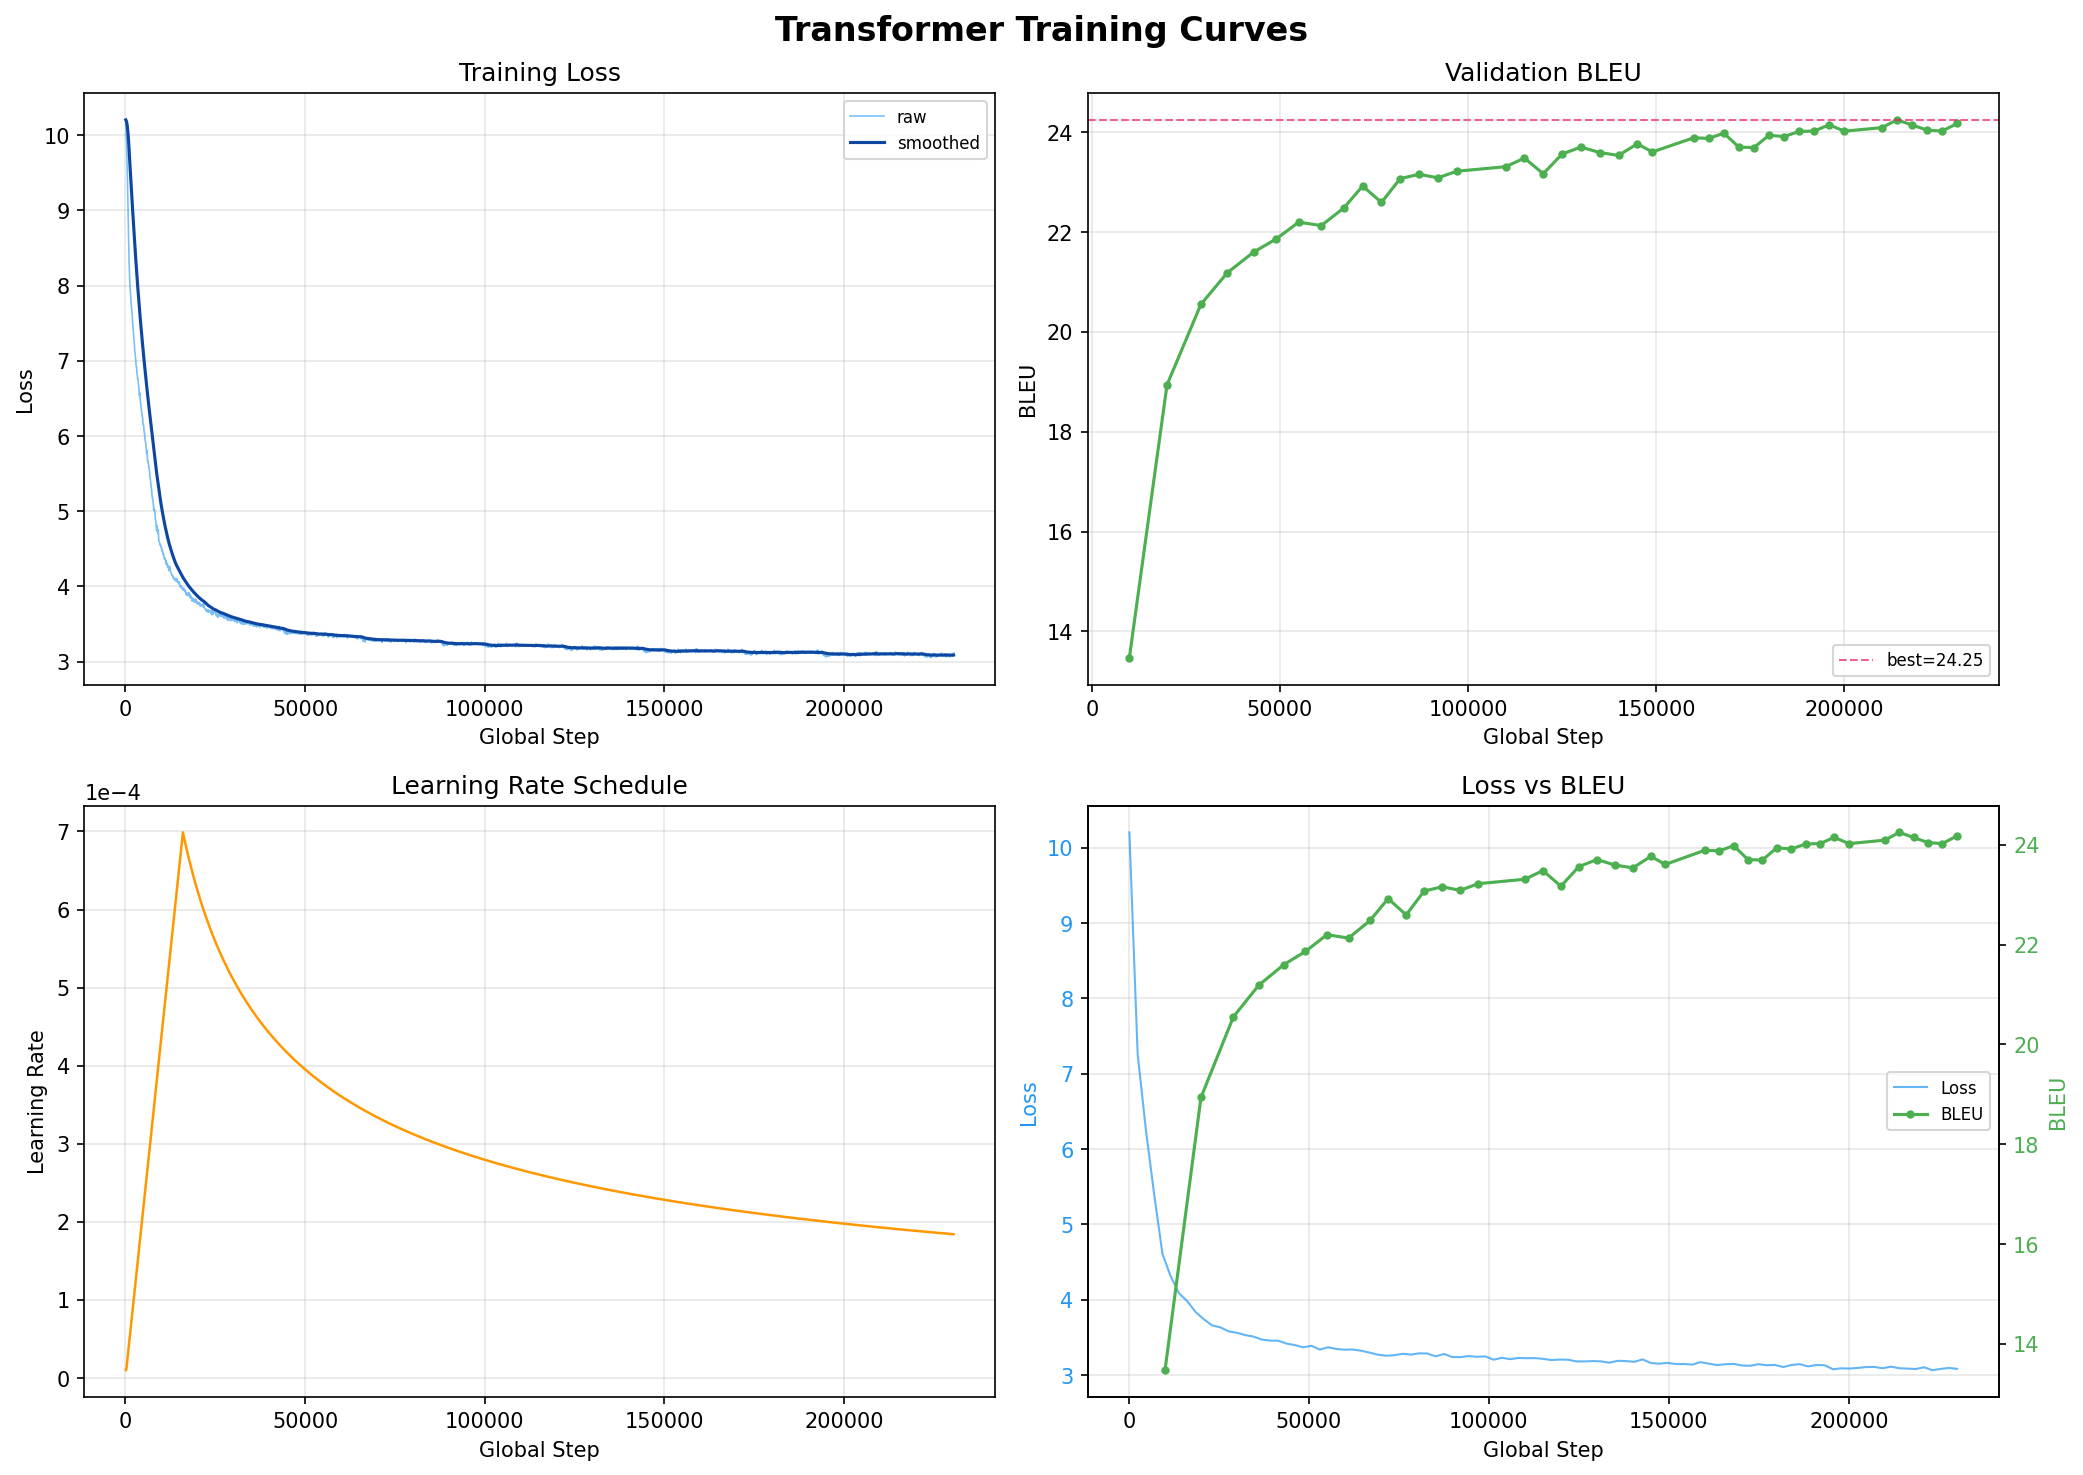
\includegraphics[width=\columnwidth]{figures/base_ende_curves.png}
\caption{Base en-de training curves (60M parameters, 230K steps, 4.17M strict-filter en-de corpus). Validation BLEU climbs monotonically through 24.25 by step 214K and plateaus thereafter. The valid/test gap is narrow (24.35 / 24.04 averaged, $-0.31$) consistent with newstest2013 and newstest2014 being similar-difficulty en-de news distributions.}
\label{fig:base_ende_curves}
\end{figure}

\subsection{Big en-de}
Big en-de trains for 466K steps with dropout 0.3 (the original Vaswani en-de regularization); best single-checkpoint valid is 23.41, with 5-checkpoint averaged valid / test 23.01 / 22.47.

\subsection{The pattern replicates}
\begin{table}[t]
\centering
\small
\begin{tabular}{lrrr}
\toprule
\textbf{en-de} & \textbf{Base (60M)} & \textbf{Big (209M)} & \textbf{$\Delta$ (Big$-$Base)} \\
\midrule
Valid & 24.35 & 23.01 & $-1.34$ \\
Test  & 24.04 & 22.47 & $\mathbf{-1.57}$ \\
\bottomrule
\end{tabular}
\caption{en-de results on newstest2013 (valid) / newstest2014 (test). sacrebleu 13a, beam=5, length-penalty=1.0, 5-checkpoint averaged. \textbf{Big falls below Base by $-$1.57 BLEU on test} and $-$1.34 on valid. The capacity gap is wider than en-fr v2's $-0.87$, consistent with --- but not necessarily caused by --- the smaller effective corpus.}
\label{tab:ende}
\end{table}

The Base $>$ Big ordering on en-de matches the direction of en-fr v2's $-0.87$, with a larger magnitude ($-1.57$ on test). The two may differ mechanistically: en-fr v2 fails through data \emph{noise}, while en-de plausibly fails through data \emph{quantity}, since 4.5M en-de is genuinely cleaner per-pair (\S\ref{sec:setup}) than 30M en-fr v2 yet $\sim$~half the size of clean v1.1's 9.3M. Both routes yield Base $\geq$ Big.

A unifying \emph{hypothesis} consistent with the three data points so far is that Big requires both (a) cleanly-aligned data and (b) enough of it: v1.1 has both, v2 has (b) but not (a), and en-de has (a) but not (b). Three points do not establish a curve, and we avoid claiming a precise scale threshold; we only note that the en-de result is consistent with this picture. A cross-language scaling sweep with multiple corpus-size points per language would be needed to test the hypothesis directly.

\subsection{HuggingFace release}
Both en-de checkpoints are published on the HuggingFace Hub:
\texttt{euswbnix/transformer-wmt14-ende-base} (60M, test 24.04) and
\texttt{euswbnix/transformer-wmt14-ende-big} (209M, test 22.47).
